\def\year{2015}
\documentclass[letterpaper]{article}
\usepackage{aaai}
\usepackage{times}
\usepackage{helvet}
\usepackage{courier}
\usepackage[dvipdfmx]{graphicx}
\usepackage{amsmath}
\usepackage{amsfonts}
\frenchspacing
\setlength{\pdfpagewidth}{8.5in}
\setlength{\pdfpageheight}{11in}
\pdfinfo{
/Title (Insert Your Title Here)
/Author (Put All Your Authors Here, Separated by Commas)}
\setcounter{secnumdepth}{0}
\begin{document}
%
\title{Gaussian Processes for Modelling of Crowds}
\author{CS4246 Project: Planning and Decision Making in the Real World  \\ \\
{\bf Team 04} \\
Huang Wei Ling, A0101200R\\
Nathan Azaria, A0113011L\\
Ng Hui Xian Lynnette, A0119646X\\
Nguyen Duc Thien, A0093587M\\
Oh Shunhao, A0065475X\\
}
\maketitle
\begin{abstract}
\begin{quote}
Crowd management is essential in events where the committee has to plan and organize in an effective and efficient manner, taking into consideration factors such as the facility, size and demeanor of the crowd and crowd control. The motion analysis of crowd in multivariate timeseries data requires an effective model to represent the data. In this report, we illustrate the use of Gaussian Processes to model crowd distributions from noisy and unevenly-sampled position data, and we explore how this representation can be used to predict the density of the population for future data.
\end{quote}
\end{abstract}

\section{1.  Introduction}
In this report, we propose the use of Gaussian process for modelling of crowds. Particularly, we will discuss how we exploit the desirable properties of Gaussian process model, some of the advantages that the model provide, the critical requirements of our proposed application as well as how people can make use of the results of our analysis to plan and make decisions for future crowd controlling or crowd management. Next, we will touch on the technical details which includes the fitting on the characteristics of Gaussian process model for the application, additional findings we gathered and modification of the model to enhance performance. The third section of the report will be a detailed experimental plan we will be using to perform and evaluate the performance of Gaussian process(GP) for modelling of crowds. Lastly, the report will end with an interesting factor we will be exploring in this project.

\section{2.  Gaussian Process Regression for Motion Analysis of Crowds}

{\bf2.1  Constructing Mean and Covariance Functions} \\

In a Gaussian Process model, we model a target variable $f(x)$ as a function of the input locations $x \in X$. The sensor readings $y$ of $f(x)$ at each point $x$ is expressed in the form $y = f(x) + \epsilon$, where each $\epsilon \sim \mathcal{N}(0, \sigma^2)$ is an i.i.d. additive noise term. $y$ is expressed with a Gaussian Process distribution as follows:

\begin{center}
$y = f(x) \sim GP(m(x), k(x,x^\prime))$
\end{center}

where $m: X \rightarrow \mathbb{R}$ is the mean function of the distribution and $k: X \times X \rightarrow \mathbb{R}$ is a kernel function which describes the covariances between the values of $y$ any pair of values of the independent variable, $x$ and $x^\prime$ in $X$. \\

In our Gaussian Process model, each individual is modeled with a separate Gaussian Distribution. For each person in the data, the $x$, $y$ and $z$ of coordinates of the person is given at various points of time. As we seek to model the locations of each person as a function on time, the input location space (dependent variable) for our data $X$ is the time interval in which the data resides, and the target variable is the position of the person, expressed as a tuple $(x,y,z)$ in $\mathbb{R}^3$. \\

We use a heteroscedastic model that works the same way as a Gaussian Process model. However, this model allows the use of different variances for the noise terms of the observations, $\epsilon_i \sim N(0, \sigma_i^2)$, giving different weights to each observation. Therefore, it serves to fit observations with smaller noise and choose to ignore those with larger noise. \\

By experimenting with different kernel functions, we obtain the final GP model using a linear combination of a Multilayer Perceptron (MLP) and a constant Bias as kernel function as they consistently output acceptable results for regressions on our dataset. MLP, also known as arc sine kernel or neural network kernel, can be optimized to represent a complex non-linear function. \\

{\bf2.2  Qualitative Advantages} \\

There are many advantages to using the Gaussian Process model. One key property of the data is that it is unevenly sampled, with multiple large gaps in between the position readings $(x,y,z)$ of each individual. As these points are discrete and finite, the crowd densities at certain positions and times are not represented by the data. After processing the data with using the Gaussian Process model, we will be able to fill in these gaps in data. \\

Another benefit is that the Gaussian Process model provides both the mean and variances of the position of the user at each point of time, allowing us to construct a probability distribution of the user's position at each point of time. A probability distribution allows us to compute the proportion of the crowd at any point of time, over any defined region. \\

One reason why this model is a good fit is because of the correlation between the current position of each individual and the future positions. Thus the coordinates of the individuals each modelled as a trajectory over time. There have been past usages of the GP model trajectory prediction in data. For example, in a paper by {\it Marco A. F. Pimentel, David A. Clifton, Lionel Tarassenko}, Gaussian Processes were used to model the trajectory of human vital signs. \\

Gaussian process model fits our application well as we can can specify the variance of noise at each point and deal with gaps between data if there is a break in between the event or if the event spans multiple days. The usual approach to interpolating between is through traditional curve-fitting algorithms like the cubic spline. However, these methods do not cater to noisy data as well as Gaussian Processes do, and unlike Gaussian Processes, do not provide a probability distribution (through mean and variance values) at each point of time, which is important for our method of integrating over regions we are interested in to obtain expected crowd densities.\\


{\bf2.3  Important Requirements} \\

% Some repeated information from Section 4.2 "Real world dataset"? I think we shouldn't talk about our dataset here. here is for general datasets
Some of the important requirements of crowd modelling include the use of big data and the data of different demographics of people and locations in the building. One benefit of the dataset is that we are able to locate the participants at each point of time, allowing us to collect datapoints due to the use of time axis. As the number of participants is large, we can perform Gaussian process on all of them and the datapoints can be distributed. \\

Gaussian process models are a non-parametric Bayesian approach to regression and classification and we consider these models with multivariate outputs. Our dataset uses a simple multivariate model which applies a separate GP to each dimension, thus assuming statistical independence between the output dimensions. The statistical independence can be supported by parallel GP models. However, actual multivariate observations are likely to have significant correlation and structure. Thus, one possible improvement to achieve GP models with correlated output can be formed by passing the independent GP priors through a function, such as multi-class classification, as stated in a paper by {\it Antoni B.Chan} on the topic of Multivariate Generalized Gaussian Process Models. \\


{\bf2.4  Interpreting Outputs} \\

After modelling the trajectories of each person as a function of time, point of time $T$, for each person $i$, we can determine the mean vector $\boldsymbol{\mu}$ and covariance matrix $K$ of the person's $x,y,z$ coordinates. Let $U_i$ be a random variable denoting the position $(x,y,z)$ of person $i$. Each $U_i$ can then be expressed as a trivariate normal distribution $U_i \sim \mathcal{N}(\boldsymbol{\mu},K)$.\\

To compute the expected amount of people in a region $R$, we define the indicator variables for each $i \in \{1,2,\cdots,n\}$:
\begin{center}
$X_i =
\begin{cases}
    1 &\text{if user }i\text{ is in region R}\\
    0 &\text{otherwise}
\end{cases}$
\end{center}
The expected value of $X_i$, is equal to the probability of person $i$ being in region $R$, which is computed as $\int_R p_i(x,y,z)dV$, where $p_i(x,y,z)$ is the probability density function of $U_i$. Thus, the total number of people in region $R$ is $\sum_{i=1}^n X_i$, with an expected value:
\begin{center}
$\displaystyle E[\sum_{i=1}^n X_i] = \sum_{i=1}^n E[X_i] = \sum_{i=1}^n \int_V p_i(x,y,z)dV$.
\end{center}

However, in our experiment, we do a simplified version, using independent Gaussian Process models for each of the axes $x$, $y$ and $z$, thus the covariances between any two variables to be $0$. \\

Thus using simple integrations over regions, we can compute the expected number of people in each region. The outputs of the Gaussian Process model are useful in helping human users or experts in using a sample of people in the data to predict the population density of a particular area at any instance of time. The idea is we can tag a small group of people and they will conduct their activities as per normal. We will get the datapoints of their movements to evaluate the GP model and get the distribution so as to predict the expected population density of a particular area at any instance of time. \\

\section{3.  Technical Approach}

{\bf3.1  Fitting the requirements using GP model} \\

%Add diagrams
input of 3 graphs \\


In order to support the use of big data and the data of different demographics, we experimented with several families of kernel functions including the Radial Basis function (RBF), Exponential function, Matern52, Matern32 and Multilayer Perceptron (MLP). The experiments conducted involved varying their respective parameters such as noise values, relaxing or fixing constraints, changing initial values and inducing points and combining with various White and Bias kernels. Finally, the combination of kernel functions that yield consistent results as observed cross different samples from our dataset is selected to build our GP model for further application. In our case, we found out that MLP with a bias is the most effective way of representing the big data that we have.\\

We extract the X, Y and Z coordinates from the GPS location and perform the regression against the timestamps provided in the dataset. We also generate a common set of timestamps to predict the user movements against, in which we generate the mean and variance from the output of the GP we had earlier regressed. \\

The experiment is conducted using Python. For the Gaussian Process modelling and regression, we use the library Sheffield GPy with the help of Scipy and Numpy for numerical calculation and representation. We use the data structure and data analysis tools provided by the module Pandas to store, access and analyze our dataset. \\

The two methods we have chosen to regress our model are either the Stochastic Variational Inference method using the climin module or the AdaDelta rule and direct optimization using BFGS method. Through observing the results from several samples of our dataset, the latter is found to provide more desirable results and more suitable to be used in our propose application. Therefore, it is chosen for further experiments. Figure \ref{fig:GP1} and Figure \ref{fig:GP2} shows the output of two such regressions for users 3056 and 3064. \\

\begin{figure}[h!]
  \centering
    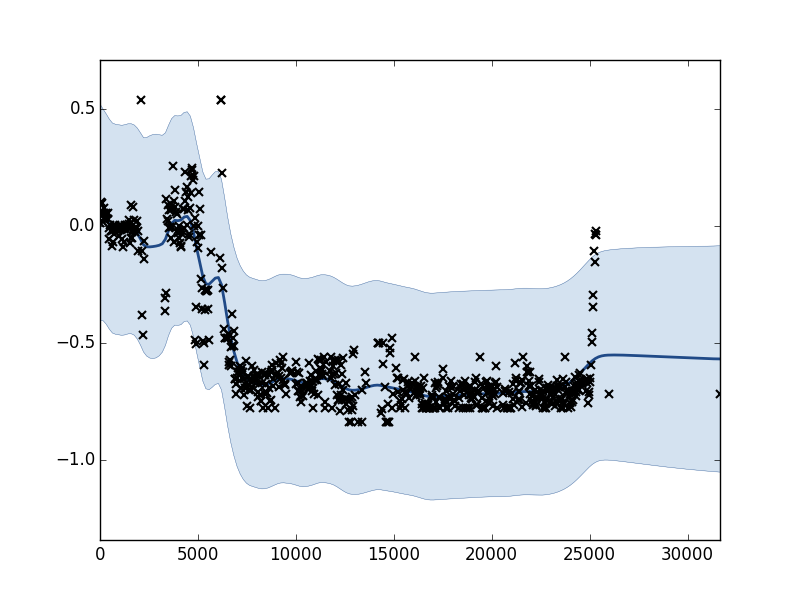
\includegraphics[width=280px,natwidth=634,natheight=442]{selected_GP/3056.csv_X.png}
  \caption{$X$ coordinates of GPS location against time stamps for User 3056 with covariance and mean derived from regression with Gaussian Process}
  \label{fig:GP1}
\end{figure}

\begin{figure}[h!]
  \centering
    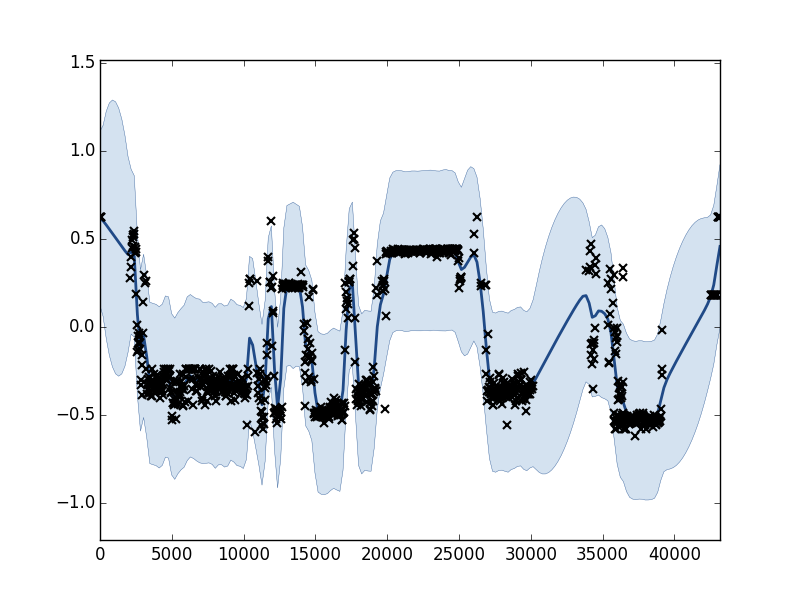
\includegraphics[width=280px,natwidth=634,natheight=442]{selected_GP/3064.csv_Y.png}
  \caption{$Y$ coordinates of GPS location against time stamps for User 3064 with covariance and mean derived from regression with Gaussian Process}
  \label{fig:GP2}
\end{figure}

{\bf3.2  Additional Insights} \\

There are several additional insights we have gathered after performing the experiment. We found out that there is little correlation between the datapoints due to the random change in GPS coordinates with respect to the timestamp as users move randomly within the conference area, and a linear regression model will not be suitable to model the data. \\

The use of the GP model in the application enables us to use all the samples and feature information to perform the prediction, while allowing the training data to have different or uneven sampling rates. Particularly, in our dataset, not all the participants have their GPS signals sampled at the same timestamps all of them might not have the same number of sample points. \\

We also noticed that the number of dimensions the dataset have will affect the computational efficiency as GP is not computational efficient in high dimensional spaces. Since our dataset only consists of a few dimensions, each GP model takes less than a minute to compute on average with the longest taking approximately 3 minutes.\\

Be default we regress the $(x,y,z)$ coordinates of each individual as it is convenient to use and easy to understand (and integrate over). However, an issue with $x$, $y$ and $z$ coordinates is that they may not be a very good model of crowd densities, especially for less open spaces. In our dataset, because the event is a conference, the spaces are wide open, this is not an issue as individuals with close together $x$, $y$ and $z$ coordinates are likely to be close to each other as well. However, in buildings with narrower corridors and tighter spaces, individuals with similar $x$, $y$ and $z$ coordinates may actually be very far apart from each other. Figures \ref{fig:opspace1} and Figure \ref{fig:opspace2} illustrate this idea.

\begin{figure}[h!]
  \centering
    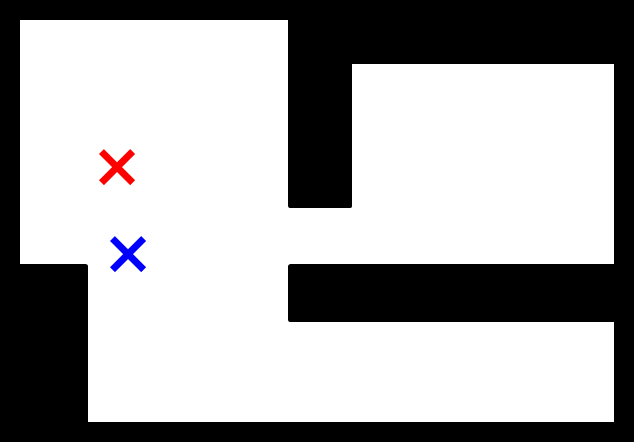
\includegraphics[width=150px,natwidth=634,natheight=442]{openspace1.png}
  \caption{Points with similar $x$ and $y$ coordinates in an open space}
  \label{fig:opspace1}
\end{figure}

\begin{figure}[h!]
  \centering
    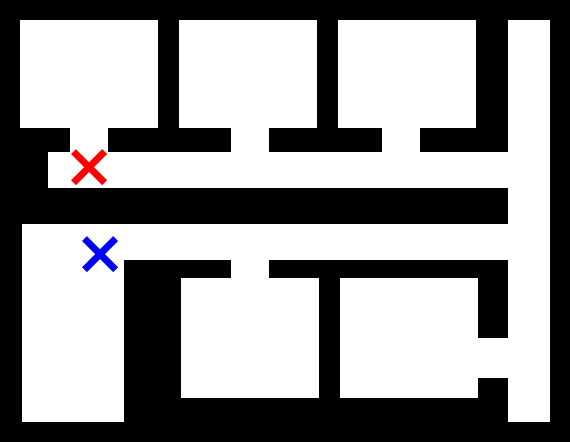
\includegraphics[width=150px,natwidth=570,natheight=442]{openspace2.png}
  \caption{Points with similar $x$ and $y$ coordinates in a less open space}
  \label{fig:opspace2}
\end{figure}

{\bf3.3  Improvement} \\

% What is this for?
By knowing the predicted densities of people within a defined radius of a certain point, we can do better crowd control. For example, given a prediction that people tend to crowd around a certain area at a certain point of time, obstacles can be reduced or shifted about. Personnel can also be deployed to facilitate crowd movement. This will be useful in cases of MRT breakdowns. \\

% What is this for?
In addition, by being able to predict the crowd density of an area in a future timestamp, we can do a certain form of path prediction. This can help in deciding building maps and object placements. For example, if we can model that generally if the crowd density of the facial shop increases, generally the crowd density of the restrooms will increase in the next timestamp, we might want to consider putting the restrooms in near proximity to the facial shop. Or if we can model that the crowd density streams from one product to another in a supermarket, we might want to consider placing both products near each other so shoppers can easily reach for both products at once, hence increasing the sales revenue.  \\

\section{4.  Experimental Evaluation}

{\bf4.1  Real-World Dataset} \\

We test our approach using a Attendee Meta-Data (AMD) Hope RFID Dateset from which data is collected from 1224 hackers attending The Last HOPE Conference from 18-20 July 2008, located in Hotel Pennsylvania, New York City. The data set details the location of the people through the use of RFID badges that uniquely identify and track them across the conference space over the course of the conference. \\

This dataset was used as it has some convenient properties which allow us to construct an experiement to test our model.\\

Firstly, the position data is usually taken at regular intervals of about $30$ seconds apart. Secondly, the data provided is exhaustive (as each attendee to the conference is tagged). Thus the data provides enough information to find the number of people in each region at any point of time, by simply counting the number of people within the region, in a time window of $[t-15,t+15)$, where $t$ is the target point of time. \\

{\bf4.2  Experimental Setup} \\

In the experiment, we first divide the conference area into $8\times 7 \times 2$ square regions (on the $x$,$y$ and $z$ axes respectively) that tile the conference area. We then select $50$ different time points to test on. These data points are picked randomly, while ensuring a minimum of $200$ seconds between any two time points, and that there are at least $300$ unique active tags at that time point (measured by counting the number of tags with a data point in the region $[t-15,t+15)$, where $t$ is the candidate time point). This is done as the event spans multiple days, and there are periods where no or few people are active, like during the night.\\

At each of the chosen time points, we then count the number of unique tags within each of the $112$ regions. This is the actual data which we will be comparing against. We then take a small fraction (about $10\%$) of the people, and use the Gaussian Process model above to estimate the number of people within each of the regions (note that since we are using only $10\%$ of the data, we need to multiply the final output values by $10$ so that the output data will be on the same scale as the actual data. \\

Figures \ref{fig:t1dist} to \ref{fig:t4dist} the between the density plots between actual crowd densities and the predicted crowd densities. One way of testing the quality of the fit is by observing how the distributions differ in the plotted charts below. A more empirical way of testing the quality of the fit is by taking the mean-squared error of the data between the actual and the predicted number of people. This can be compared across different models to test how well the data fits. \\

\begin{figure}[h!]
  \centering
    
\includegraphics[width=150px,natwidth=320,natheight=280]{selected_renders/0_1216437924.png}
  \caption{Actual distribution of people at time $t=1216437924$, first floor}
  \label{fig:t1dist}
\end{figure}

\begin{figure}[h!]
  \centering
    
\includegraphics[width=150px,natwidth=320,natheight=280]{selected_renders/0_1216437924p.png}
  \caption{Predicted distribution of people at time $t=1216437924$, first floor}
  \label{fig:t2dist}
\end{figure}

\begin{figure}[h!]
  \centering
    
\includegraphics[width=150px,natwidth=320,natheight=280]{selected_renders/1_1216440525.png}
  \caption{Actual distribution of people at time $t=1216440525$, second floor}
  \label{fig:t3dist}
\end{figure}

\begin{figure}[h!]
  \centering
    
\includegraphics[width=150px,natwidth=320,natheight=280]{selected_renders/1_1216440525p.png}
  \caption{Predicted distribution of people at time $t=1216440525$, second floor}
  \label{fig:t4dist}
\end{figure}


{\bf4.3  Other models} \\

Several types of GP models were experimented with, including Stochastic Variance Gaussian Processes and Sparse Gaussian Processes. We also performed experiments with all the different types of kernels provided by the GPy library, including linear kernel and white kernel. We also tweaked the input parameters, such as the variance of the kernels to experiment with the data. The GP model-variant that we proposed has the co-variance matrix and mean that fits the data the best. \\

To model less open spaces, we can use an alternative modelling, provided we know the layout of the area. Instead of using the $x$, $y$ and $z$ coordinates of each user, we can use shortest path distances as the attributes instead. We first define a set of reference points at significant points $p_1,p_2,\cdots,p_k$ in the area. For each data point $d$, we compute the shortest paths $s_i$ from the data point to each of the reference points $p_i$. This is shown in Figure \ref{fig:spaths}. \\

We then use the same Gaussian Process model as before using the values $s_i$ as the attributes. The advantage of using shortest paths as a metric is the geometry of the map has been abstracted out; two points with similar values of $s_i$ must be points that are close to each other. (given enough reference points)\\

\begin{figure}[h!]
  \centering
    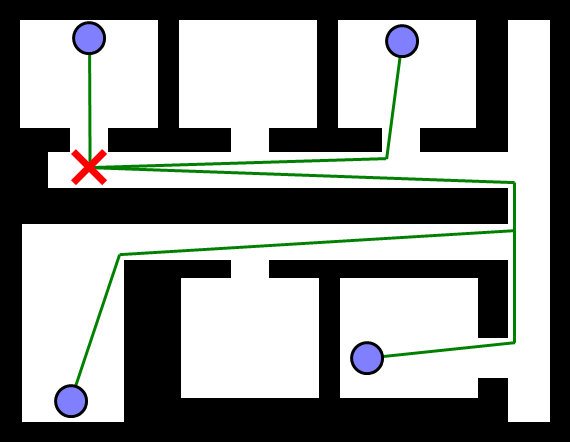
\includegraphics[width=150px,natwidth=570,natheight=442]{shortestpaths.png}
  \caption{The shortest paths from a data point to four reference points}
  \label{fig:spaths}
\end{figure}

However, it is important to note that with this formulation, the reference points must be carefully picked for a good prediction. (spread out, and preferably near the areas one is concerned about) \\

%Note: Can run the kernels that failed and put plots if needed (i.e. not enough images)

\section{5.  Conclusion}

\section{6.  References}

[1] Marco A. F. Pimentel, David A. Clifton, Lionel Tarassenko, `` GAUSSIAN PROCESS CLUSTERING FOR THE FUNCTIONAL CHARACTERISATION OF VITAL-SIGN TRAJECTORIES"
 in {\it 2013 IEEE INTERNATIONAL WORKSHOP ON MACHINE LEARNING FOR SIGNAL PROCESSING}, SEPT. 22–25, 2013, SOUTHAMPTON, UK. \\

[2] Antoni B. Chan, ``{\it Multivariate Generalized Gaussian Process Models}" NOV. 03, 2013

\section{7. Roles of Members}
\begin{enumerate}
\item Huang Wei Ling: Report Writing
\item Nathan Azaria: Crowd Modelling 
\item Ng Hui Xian Lynnette: Gaussian Process Modelling
\item Nguyen Duc Thien: Gaussian Process Modelling
\item Oh Shunhao: Mathematical Modelling
\end{enumerate}


\end{document}
